\documentclass[a4paper, 11pt]{article}
\usepackage[utf8]{inputenc}
\usepackage{amsmath}
\usepackage{amssymb}
\usepackage{listings}
\usepackage{tabularx}
	\newcolumntype{R}{>{\raggedleft\arraybackslash}X}%
	\newcolumntype{E}{>{\raggedleft\arraybackslash}l}%

\usepackage{float}
\usepackage{graphics}
\usepackage{placeins}
\usepackage{epstopdf}
\usepackage{graphicx}
    \DeclareGraphicsExtensions{.pdf,.png,.jpg,.eps}

% Lengths and indenting
\setlength{\textwidth}{16.5cm}
\setlength{\marginparwidth}{1.5cm}
\setlength{\parindent}{0cm}
\setlength{\parskip}{0.15cm}
\setlength{\textheight}{22cm}
\setlength{\oddsidemargin}{0cm}
\setlength{\evensidemargin}{\oddsidemargin}
\setlength{\topmargin}{0cm}
\setlength{\headheight}{0cm}
\setlength{\headsep}{0cm}

\renewcommand{\familydefault}{\sfdefault}

\newcommand{\TODO}[1]{\textbf{TODO:} #1}

\title{Advanced Systems Lab - Milestone \#2}
\author{Erik Jonsson Thoren - jerik\\}
\date{\today}

\graphicspath{{./img/}} % Specifies the directory where pictures are stored
\epstopdfsetup{outdir=./img/}


\begin{document}
\maketitle
\tableofcontents
\newpage

\TODO{1. Update graphs with 10 threads with the new data}
\TODO{2. Update graphs for 2:nd model with the new service times approximations}

\section{Introduction}
This report covers the approach taken to model the system from the first model to the final model. Some changes in regards to how the logging has been done in this milestone versus the first milestone is that in this milestone, the response-time logging has been moved to the client side which logs every individual response time for the requests made to the middleware. To measure the service-time, the time spent in each component in the middleware is measured for every individual request and logged. The experiment throughput is calculated by dividing the amount of requests made during an experiment (excluding warm-up and cool-down) divided by the time between the first request (after warm-up) to the last request (before cool-down).

\section{Experiments Measurement's Validity}
	To confirm the experiment log validity, the relationship $X=\frac{N}{R+Z}$ was applied to the experiment data. It showed that the measured response time and the measured throughput were valid. As can be seen in Table \ref{tbl:interaction-law} the relative difference is never over 0.96\%, which indicates that the measurements are valid. The difference could be caused by timing imprecisions and/or that the actual think time is larger than the programmatically specified think-time due due to the overhead, of for example logging.

\begin{table}[ch!]
	\centering
    \begin{tabularx}{\textwidth}{|E|R|R|R|l|}
    \hline
    Clients & Mean Response Time (ms) & Measured Throughput (req/s) & Theoretical Throughput (req/s) & Correlation \\ \hline
    1  & 3.05  & 325.77  & 327.87   & 100.64\% \\ \hline
    2  & 3.43  & 580.1   & 583.09   & 100.52\% \\ \hline
    4  & 4.2   & 943.3   & 952.38   & 100.96\% \\ \hline
    6  & 4.47  & 1336.25 & 1,342.28 & 100.45\% \\ \hline
    8  & 6.7   & 1192.9  & 1,194.03 & 100.09\% \\ \hline
    16 & 7.9   & 2020.33 & 2,025.32 & 100.25\% \\ \hline
    25 & 12.89 & 1935.16 & 1,939.49 & 100.22\% \\ \hline
    32 & 17.8  & 1797.6  & 1,797.75 & 100.01\% \\ \hline
    64 & 32.83 & 1947.43 & 1,949.44 & 100.10\% \\ \hline
    \end{tabularx}
    \label{tbl:interaction-law}
   	\caption{The correlation between the measured data and the interavtive response time law. In these test the clients were using 0 think time ($Z=0$).}
\end{table}

\section{Method}
	The method used for modelling the system were first to collect the service times in the middleware and performance metrics for different parameters:
	\begin{itemize}
		\item Number of client
		\item Number of middleware
		\item Number of threads
	\end{itemize}

	After this step, a simple model (Section \ref{sec:first-model}) were created. The model was evaluated for the different parameters measured in the first step and if inconsitencies were found, an analysis were done and a new iteration of modelling were done. The system is modelled as a closed product form network, and the models response time and throughput were calculated using Mean Value Analysis (MVA).

	\subsection{Load Dependent Centers in MVA}
		In the MVA algorithm it is never specified which type of queue is used. To simulate an M/M/m station, is it was replaced by a load dependent FEC (\textbf{Flow-Equivalent Center}) and the algorith demonstrated in \textbf{Box 36.1} (Rai Jain, 1991, p. 610) was used. So to simulate a M/M/m queue where each server has a mean service time $s_{M/M/m}$ ms, the service time for the FEC is set to (unit is ms):
		\[
		E[s] =
			\begin{cases}
				\frac{s_{M/M/m}}{n} 		& 1 \leq n \leq m \\
				\frac{s_{M/M/m}}{m} 		& n > m
			\end{cases}
		\]
		where n is the number of clients currently in the center.

	\subsection{Service Times}
		Several tests with different parameters were made to make sure that the service times were correctly defined in the models. 

	\subsubsection{Client Request Worker}
		The client request worker (CRW) is the component of the middleware which parses a request and also builds a response. This part of the middleware were measured to be load-independent with a mean service time of 0.1 ms.

	\subsubsection{Database}\label{sec:database-service-time}
		The database, or rather the persistence component in the middleware make up the bulk of the response time for the system. It was measured to be load dependent with respect to the number of concurrent requests. Data from tests where the number of database connections were varied, a linear relationship were measured (the queue in these test were always full, so it can be certain that all the connections always were utilized). The relationship was measured to $E[s](n_q) = 0.3598n_q + 1.554$ milliseconds, where $n_q$ is the number of concurrent requests being processed

		\begin{figure}[ch!]
			\centering
				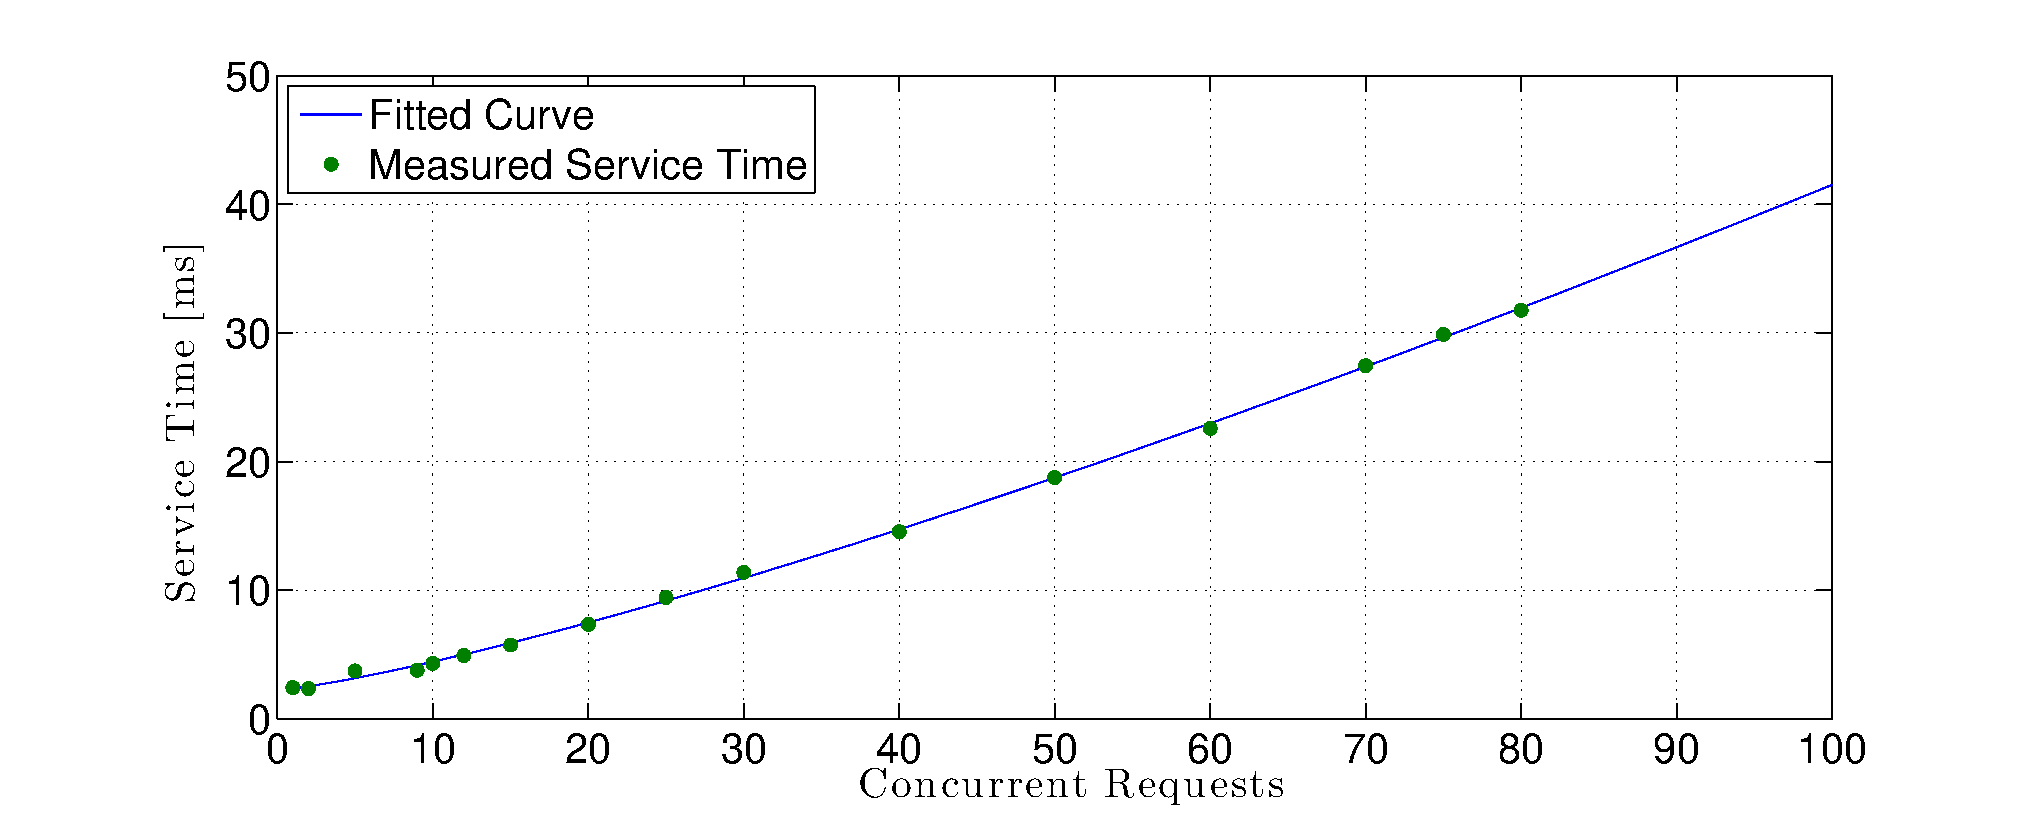
\includegraphics[width=\linewidth]{dbServiceTime}
				\rule{35em}{0.5pt}
			\caption{The service time for the database component as a function of the number of concurrent requests being processed.}
			\label{fig:db-service-time}
		\end{figure}
		\FloatBarrier

\section{First Model}\label{sec:first-model}
The first model that was designed was a closed product form network with limited population, see figure \ref{fig:firstmodel}.

\begin{figure}[ch!]
	\centering
		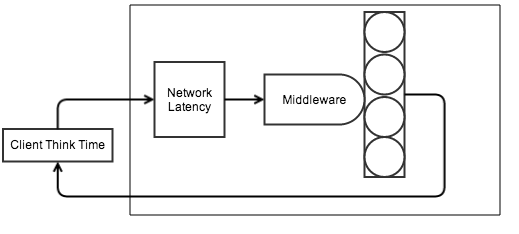
\includegraphics[width=0.8\linewidth]{firstmodel}
		\rule{35em}{0.5pt}
	\caption{Diagram over the first model applied to the system, a closed product form network.}
	\label{fig:firstmodel}
\end{figure}

\subsection{Stations}
\subsubsection{Network Latency}
The network latency in this model includes actual real network latency but also includes the time it takes for the real middleware to create a new job and insert it into the worker-threadpool queue and also to send back a response to the client. This service time was measured to be on average 1ms.

\subsubsection{Middleware}
This load dependent service center has m servers where m represents the number of worker threads. The service time for the middleware in this first attempt model is 4ms (measured from experiment using 10 worker threads) and it is load independent.

\subsubsection{Client Think Time}
This is modeled as delay center and the service time here represents the think time for the clients.

\subsection{Results}
\begin{figure}[ch!]
	\centering
		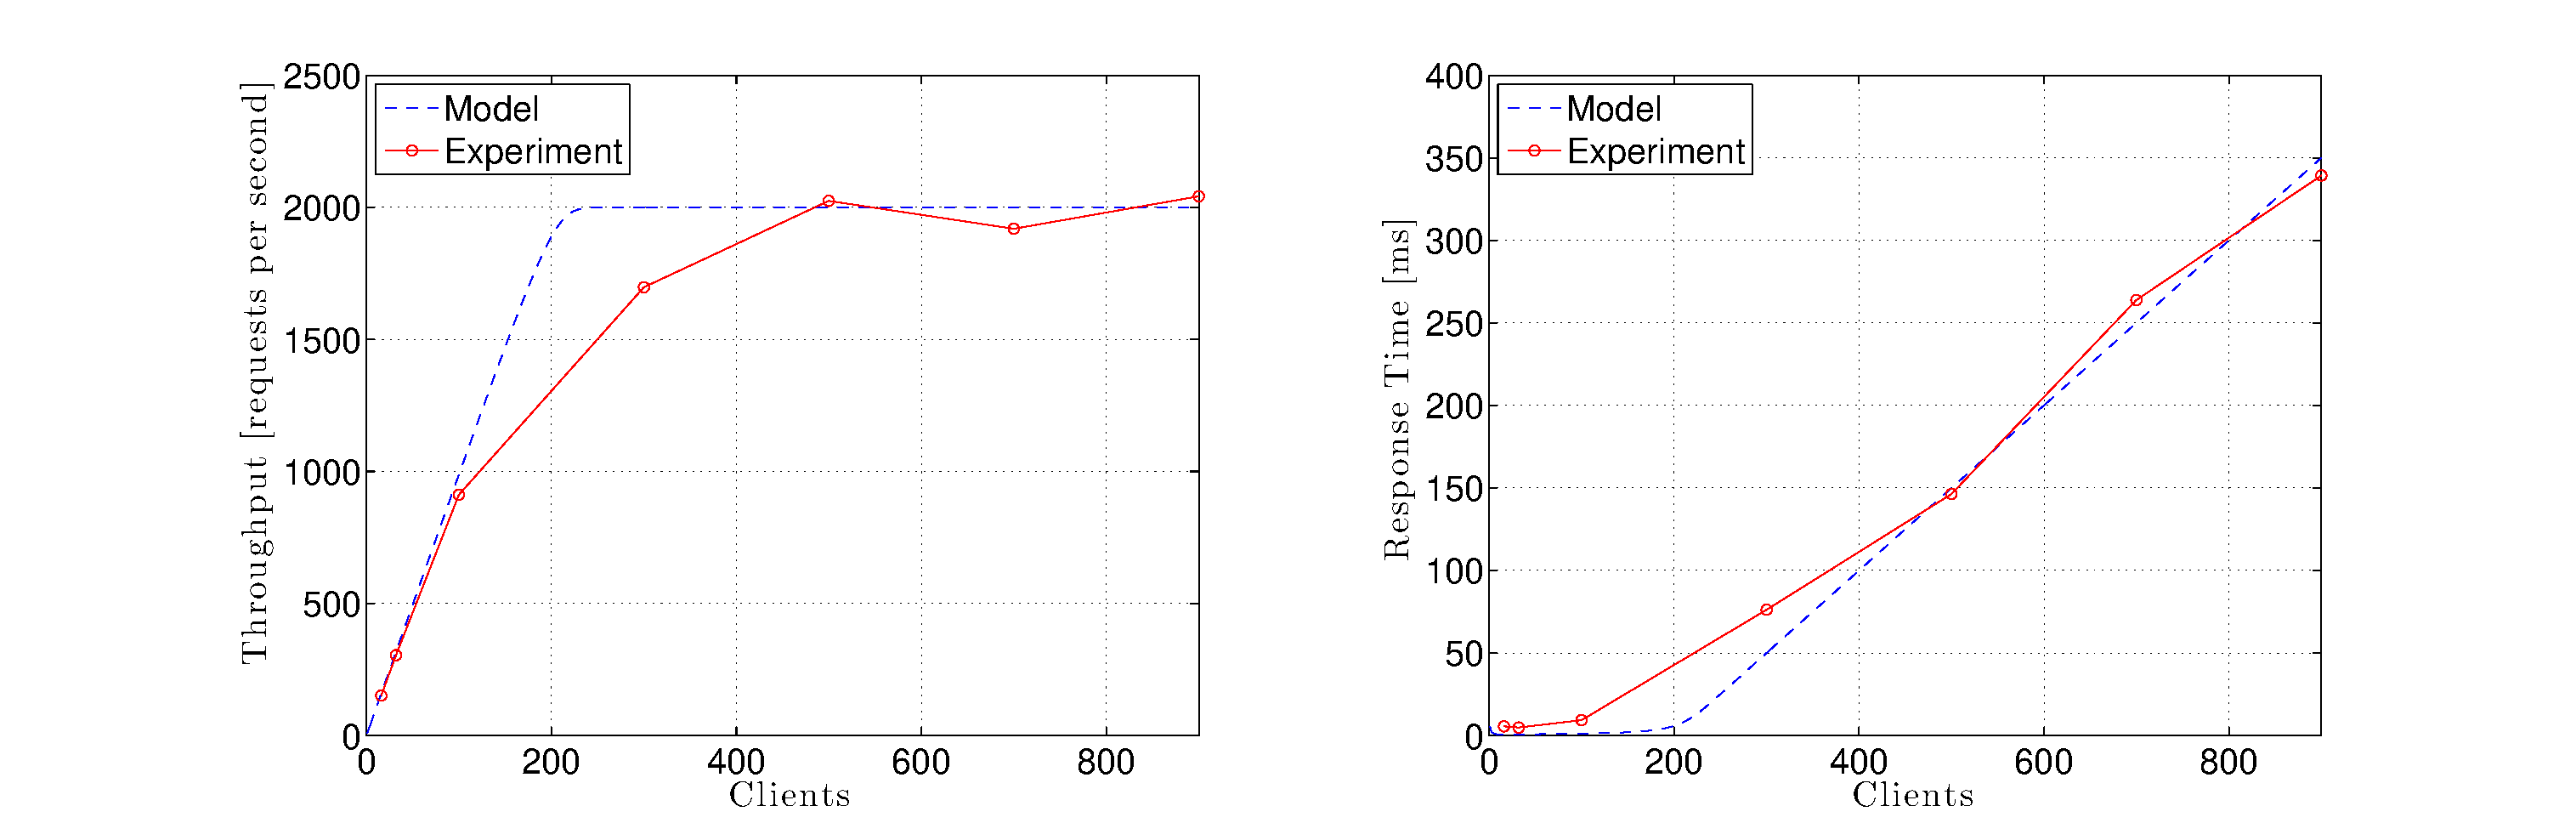
\includegraphics[width=1\linewidth,keepaspectratio]{firstRealAndModelRespAndThroughput}
	\caption{Diagram over the second model's response time and throughput compared with the experiment data of the system, using 10 middleware servers and think time of 100ms.}
	\label{fig:firstmodelResults}
\end{figure}
\FloatBarrier

\subsection{Limitations Analysis}
	The model introduced work only when using 10 middleware servers, highering the number of middleware servers will make it inconsistent with the experiment. See Figure \ref{fig:firstmodelResultsFail} for an example where this model fails. The reason for this is that in this model the middleware is modeled as a load independent station (think time 5ms) while in reality the service time is depentent on the number of concurrent requests being processed. This is caused by contention in the database. To solve this problem, a new model in created with the persitence component modelled as a load dependent station with service times as displayed in Figure \ref{fig:db-service-time} (see Section \ref{sec:database-service-time} for more information).

	\begin{figure}[ch!]
		\centering
			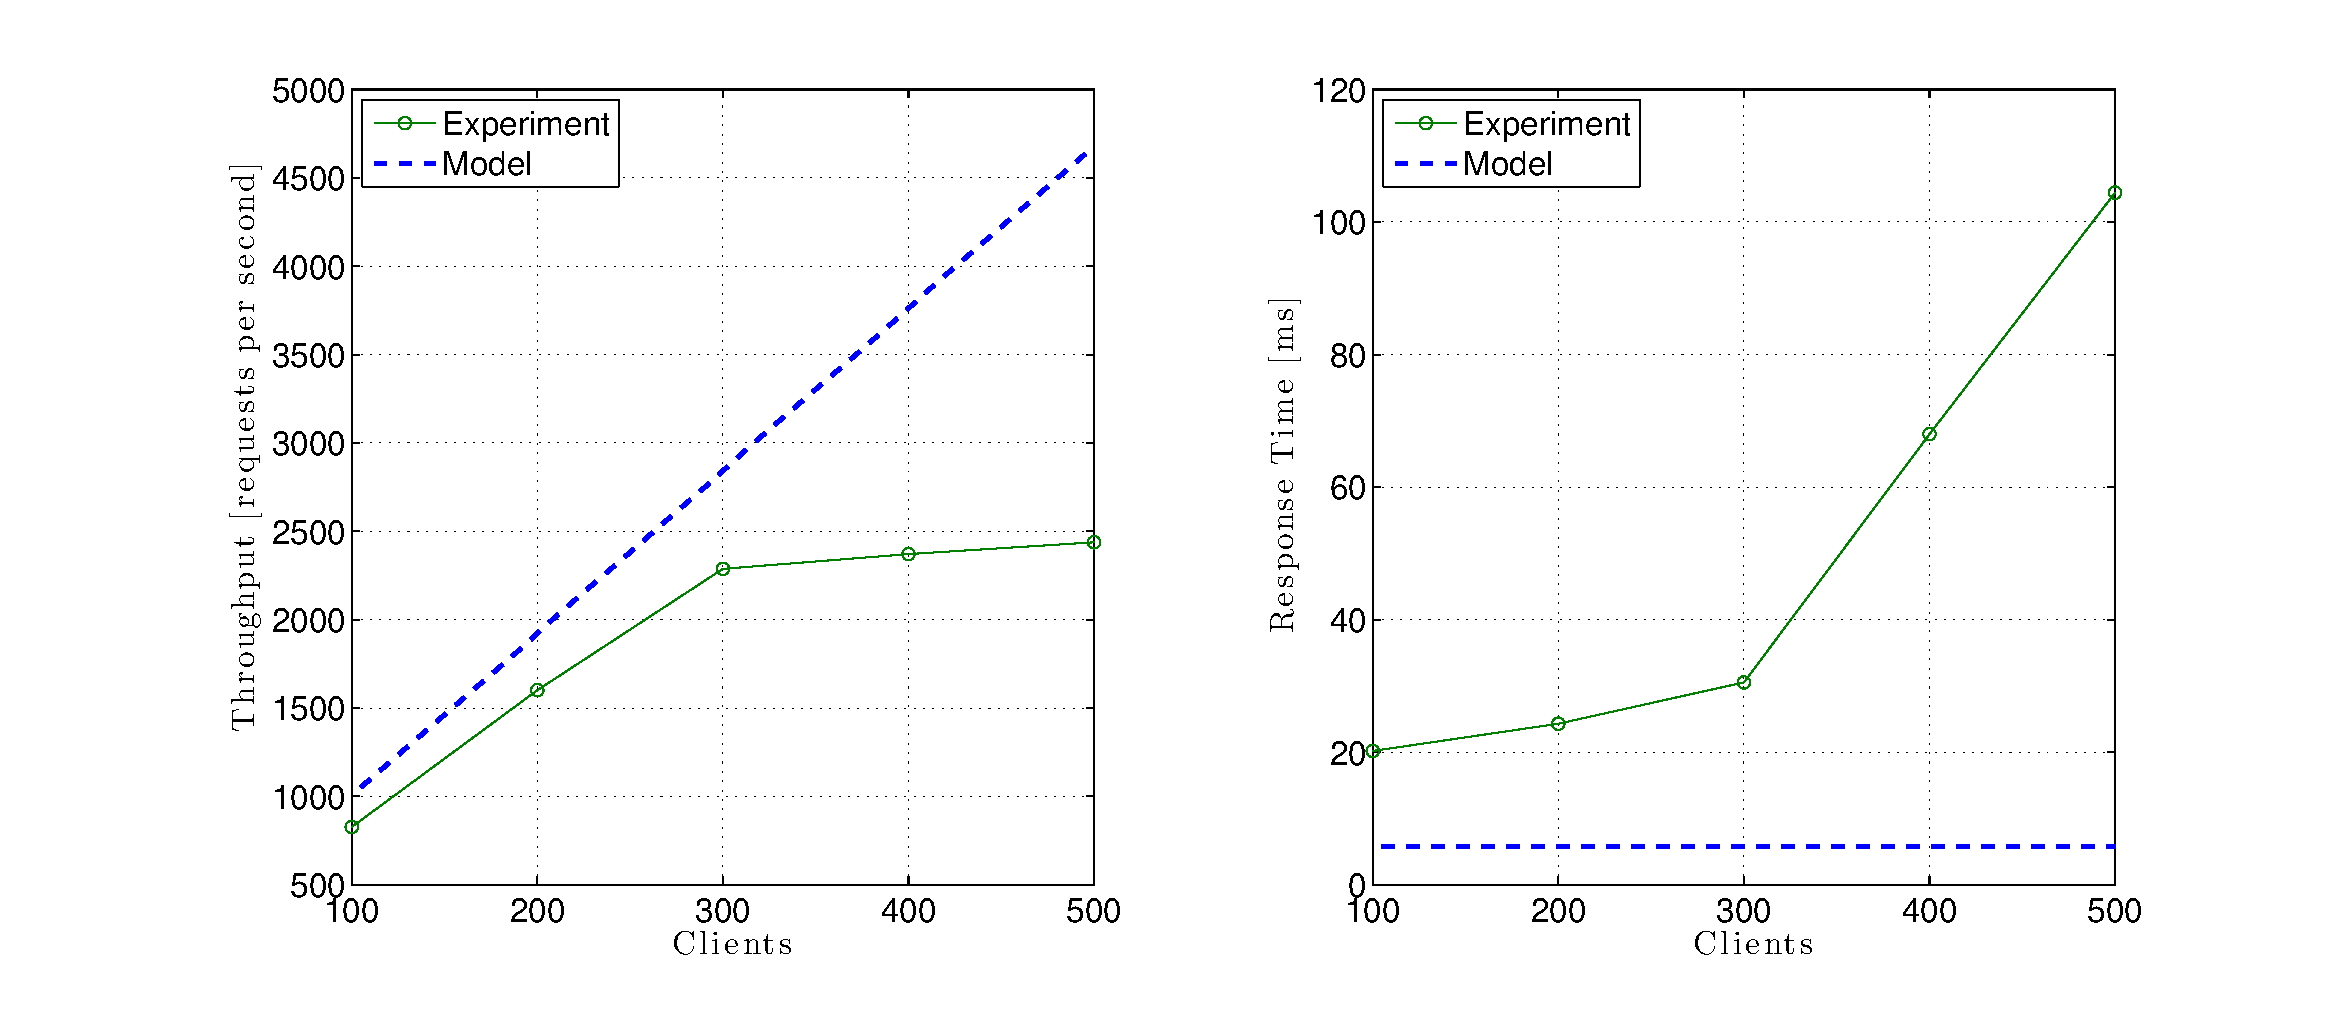
\includegraphics[width=1\linewidth,keepaspectratio]{firstRealAndModelFail}
		\caption{Diagram over the second model's response time and throughput compared with the experiment data of the system, using 80 middleware servers and think time of 100ms. The model fails to predict the actual performance of the system since in reality the middleware is load dependent.}
		\label{fig:firstmodelResultsFail}
	\end{figure}
	\FloatBarrier


\section{Introducing Load Dependency}

	The second attempt involved increasing the resolution and more importantly introducing load dependancy into the model. A diagram of the topology can be seen in Figure \ref{fig:second-model}.

	\FloatBarrier
	\begin{figure}[ch!]
		\centering
			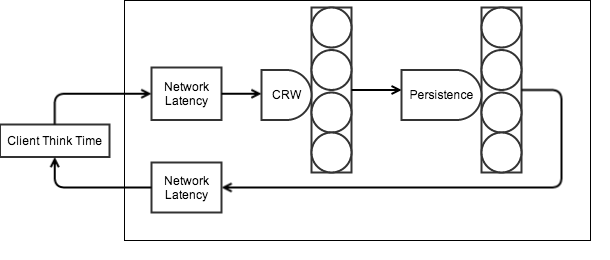
\includegraphics[width=0.8\linewidth]{secondmodel}
			\rule{35em}{0.5pt}
		\caption{Diagram over the second model applied to the system, a higher resolution model than the first attempt.}
		\label{fig:second-model}
	\end{figure}
	\FloatBarrier

\subsection{Stations}

	In this model the middleware station from the first attempt have been split into two parts: one for the client request worker component and one for the persistence component. The network latency have been split into two parts: one before and one after the client think time representing the time it takes to send to the middleware and one representing the time it takes to send a response.

	\subsubsection{Network Latency}
		This station have had it's service time halved but the number of visists have been doubled, so the total network latency is the same as the first model but is it more realistically inserted into the request flow. Modelled as a delay center.

	\subsubsection{CRW}
		The CRW is the part of the system which parses requests and build responses. This is modelled as a load independent station with service time 0.1ms.

	\subsubsection{Persistence}
		This is the most crucial change in this new attempt. The service time for this is modelled to be load dependent on the number of jobs \textit{currently being processed}; it does not depend in queue length. The service times this is modelled from can be seen in Figure \ref{fig:db-service-time}.
	
	\subsubsection{Client Think Time}
		Modelled as a delay center with constant service time that of the think time of the clients.

\subsection{Results}
	This model predicts the performance of the system much better than the first model did, this is thanks to the load dependency in the persistence component.
	\FloatBarrier
	\begin{figure}[ch!]
		\centering
			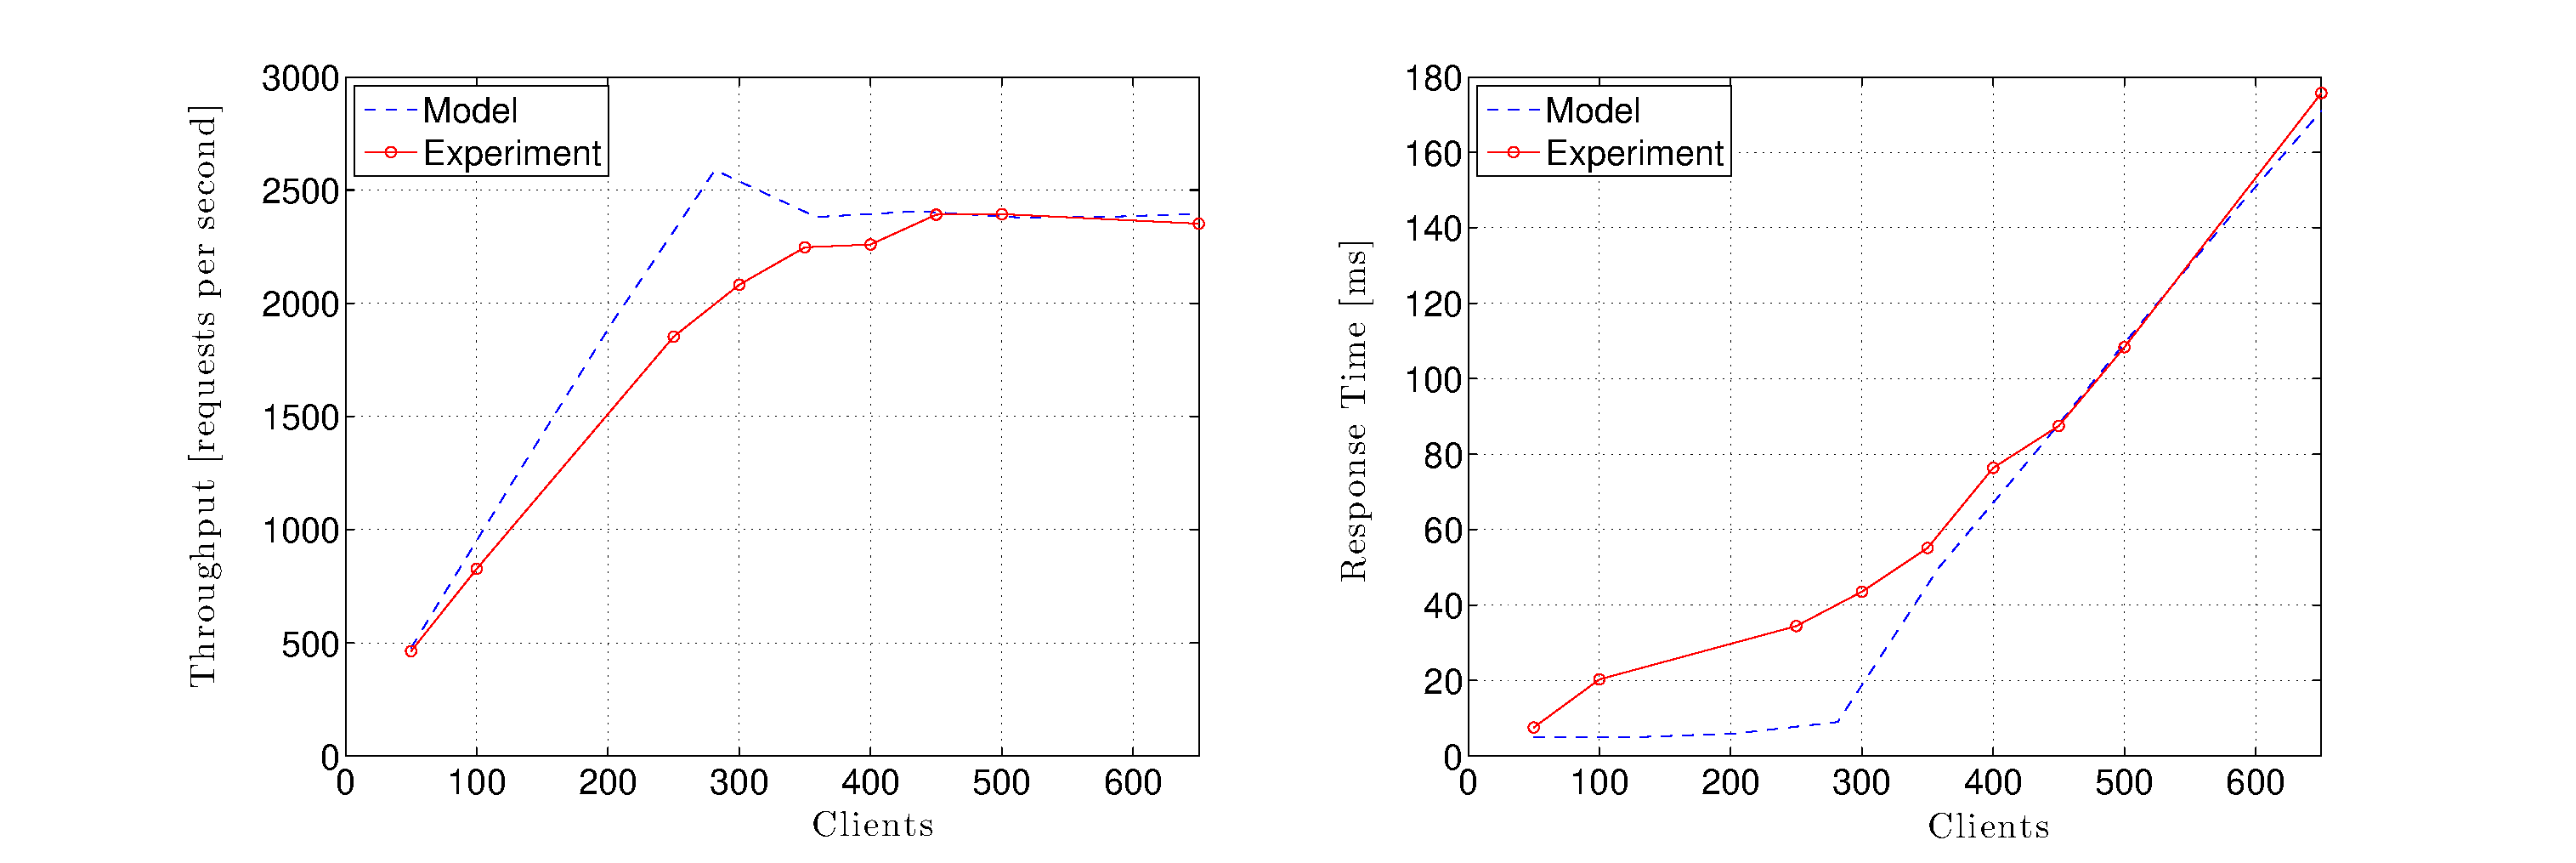
\includegraphics[width=1\linewidth,keepaspectratio]{secondRealAndModel}
		\caption{Diagram over the second model's response time and throughput compared with the experiment data of the system, using 80 CRW servers and 80 Persistence servers and think time of 100ms. This model calculates better results than the first attempt, since this model takes congestion in the database into account.}
		\label{fig:secondmodelResults}
	\end{figure}
	\FloatBarrier 
	\begin{figure}[ch!]
		\centering
			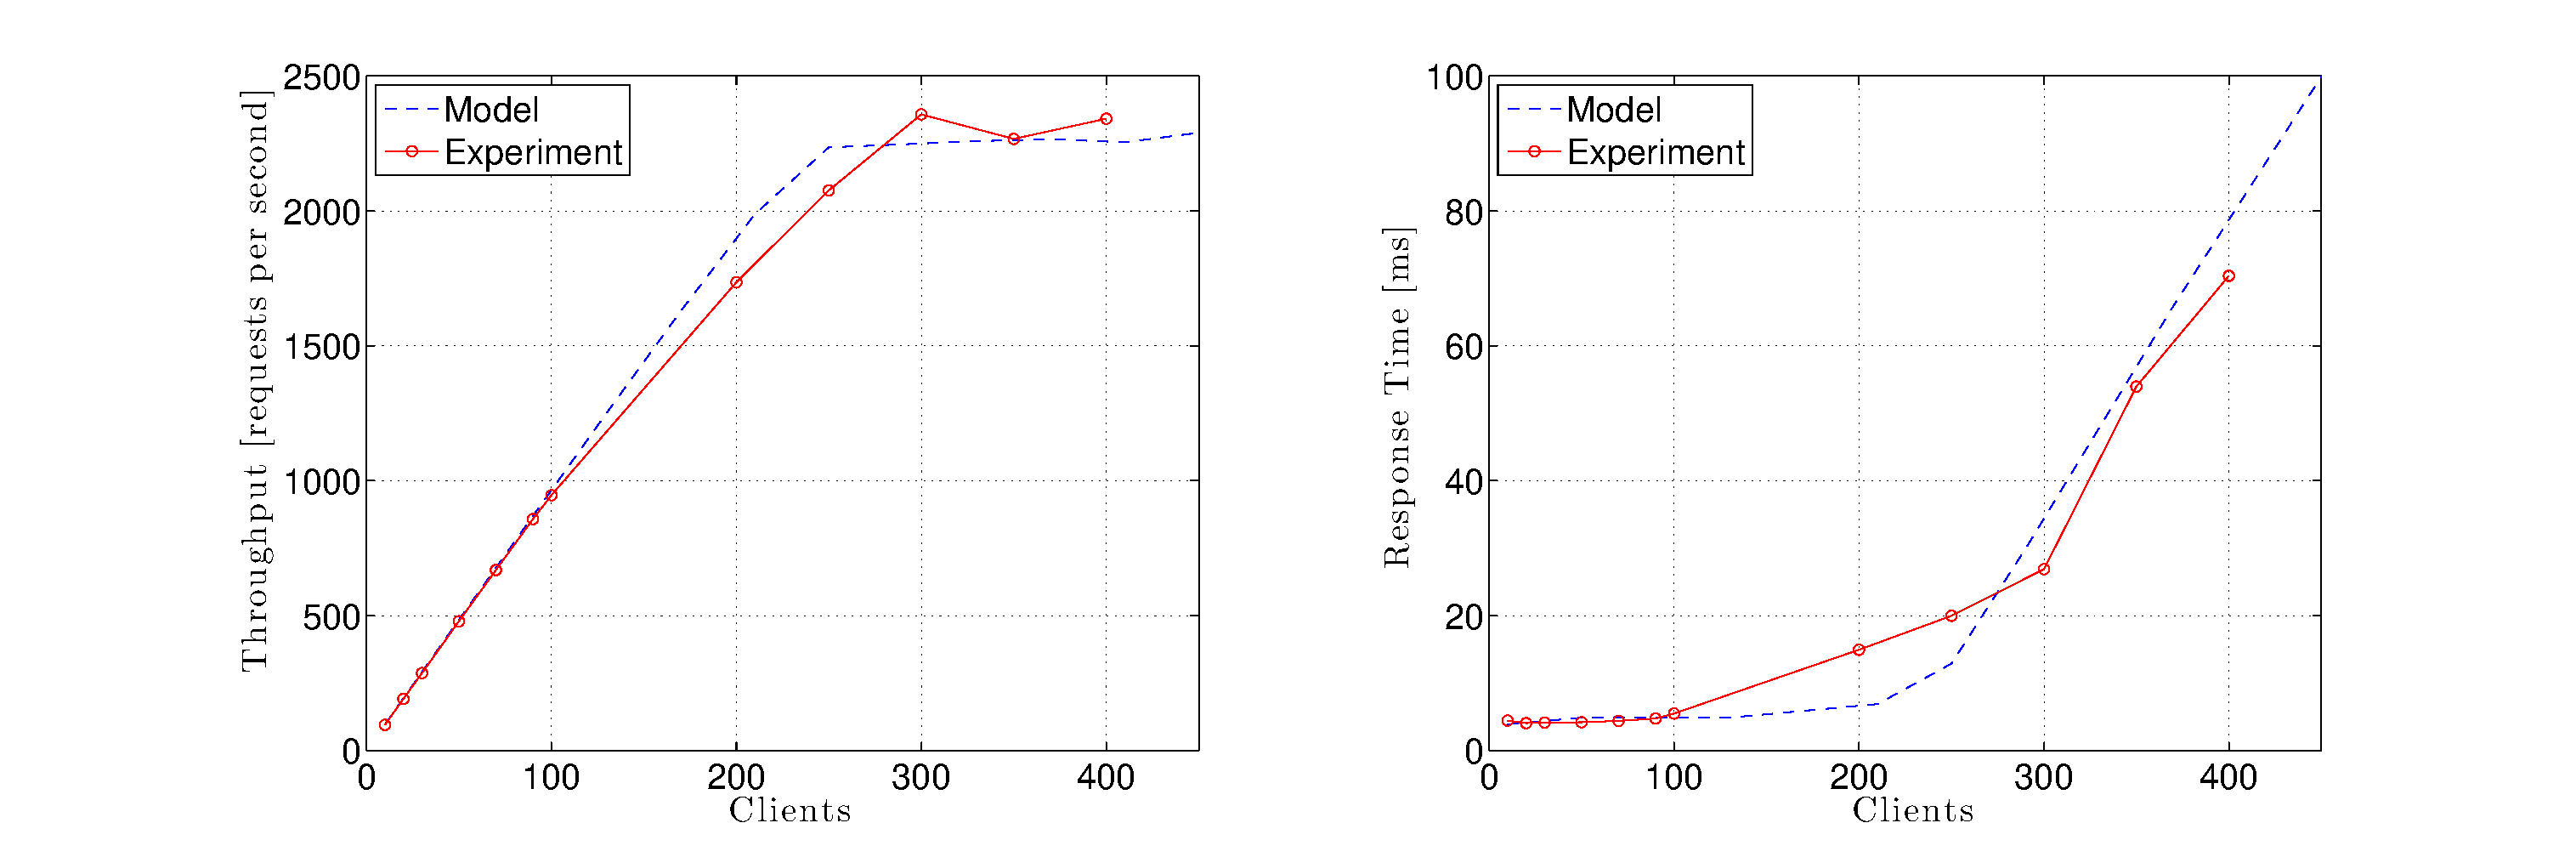
\includegraphics[width=1\linewidth,keepaspectratio]{secondRealAndModel10Threads}
		\caption{Diagram over the second model's response time and throughput compared with the experiment data of the system, using 10 CRW servers and 10 Persistence servers and think time of 100ms. Corresponds with the first model when using the same parameters.}
		\label{fig:secondmodelResults-10-th}
	\end{figure}
	\FloatBarrier
	\begin{figure}[ch!]
		\centering
			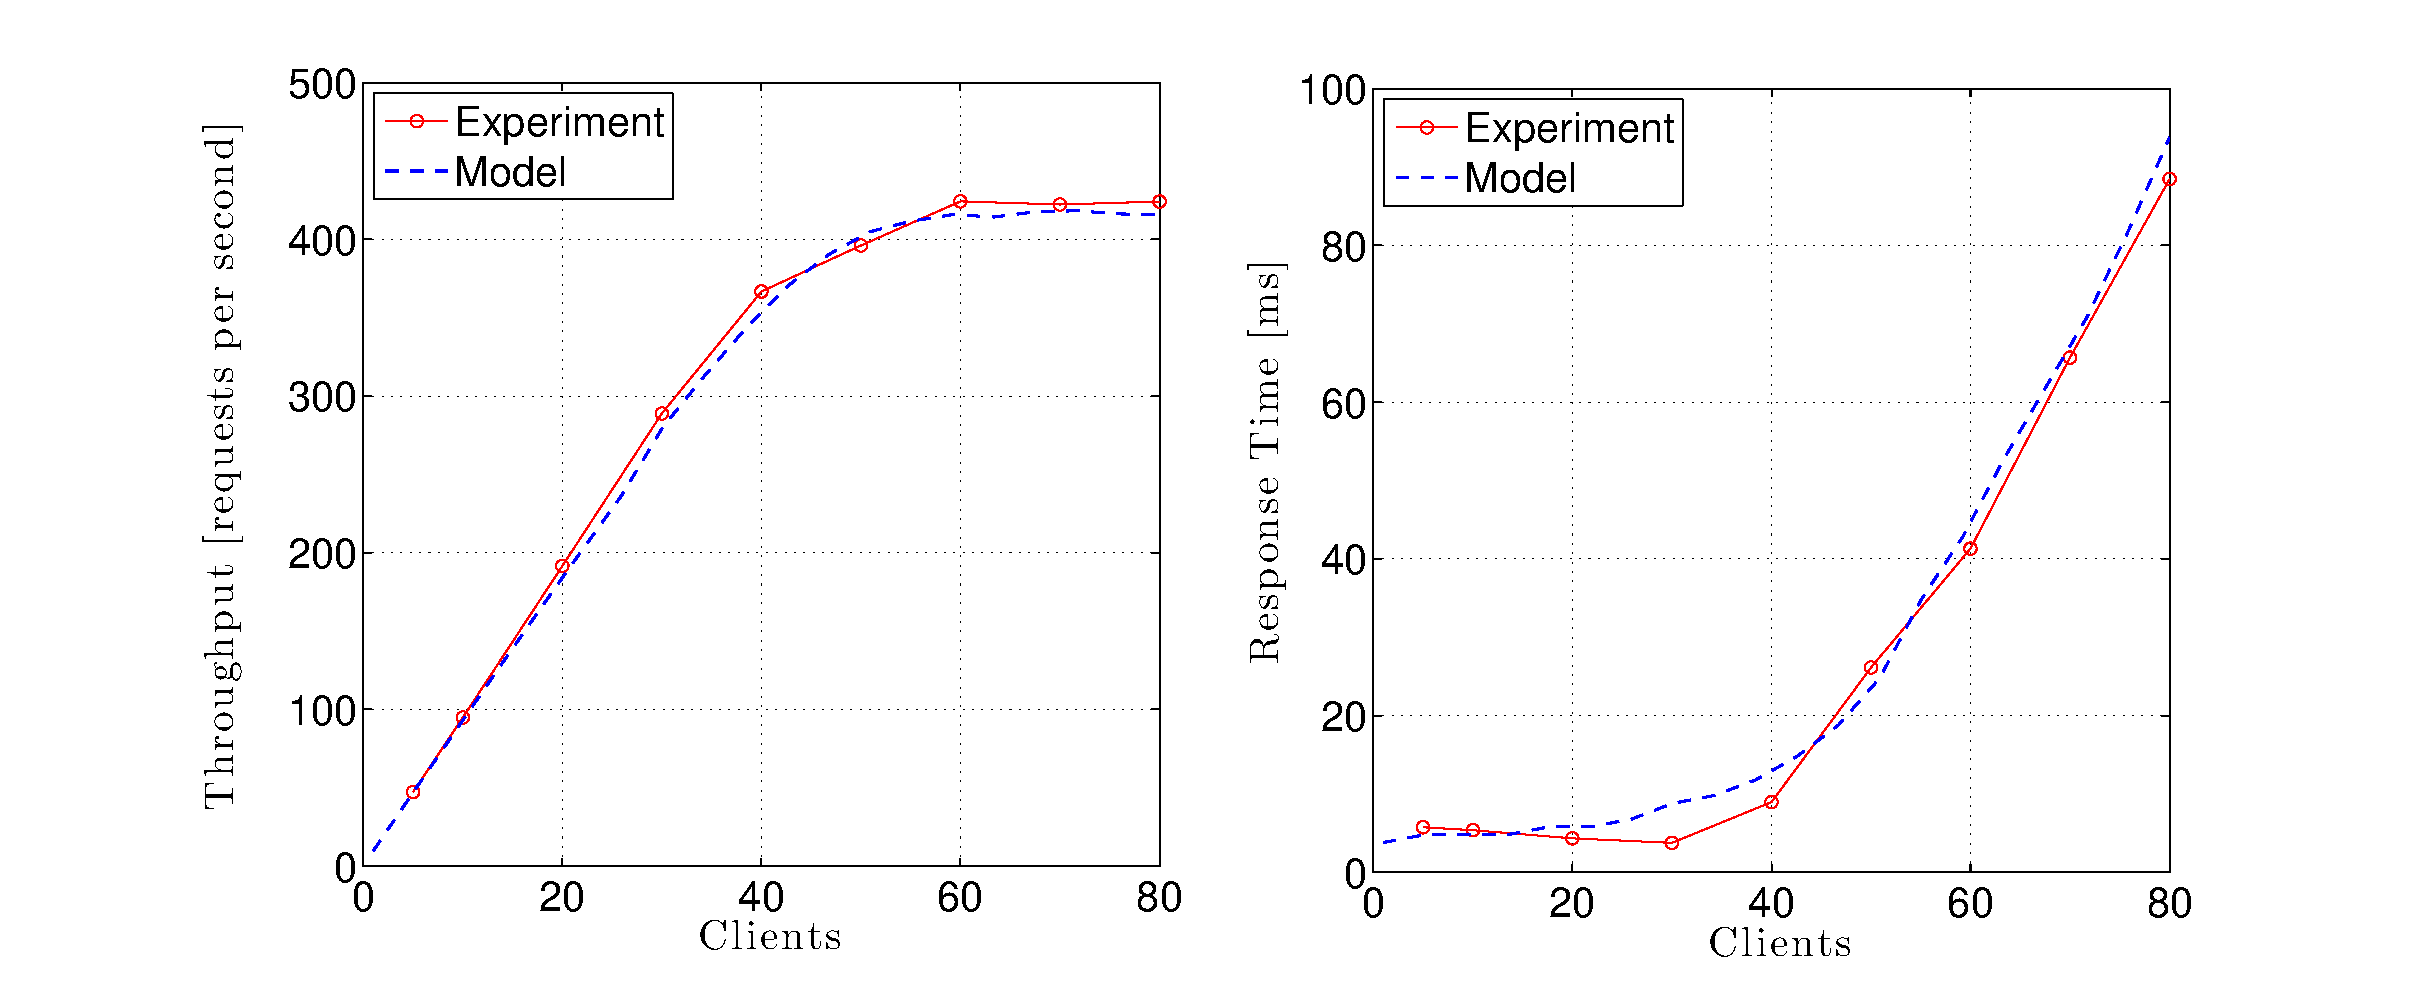
\includegraphics[width=1\linewidth,keepaspectratio]{secondRealAndModel1Thread}
		\caption{Diagram over the second model's response time and throughput compared with the experiment data of the system, using 1 CRW servers and 1 Persistence servers and think time of 100ms. Good fit with the experiment data.}
		\label{fig:secondmodelResults-1-th}
	\end{figure}
	\FloatBarrier

	\subsection{Limitations Analysis}
	The model corresponds generally well with the true performance with regards to the asymptots of response time and troughput. But before the system reaches saturation the model does not predict well when 10 worker theads, see Figure \ref{fig:secondmodelResults-error}. To get to the bottom of this discrepancy, tests were re-run for these paramaters to make sure 

	\FloatBarrier
	\begin{figure}[ch!]
		\centering
			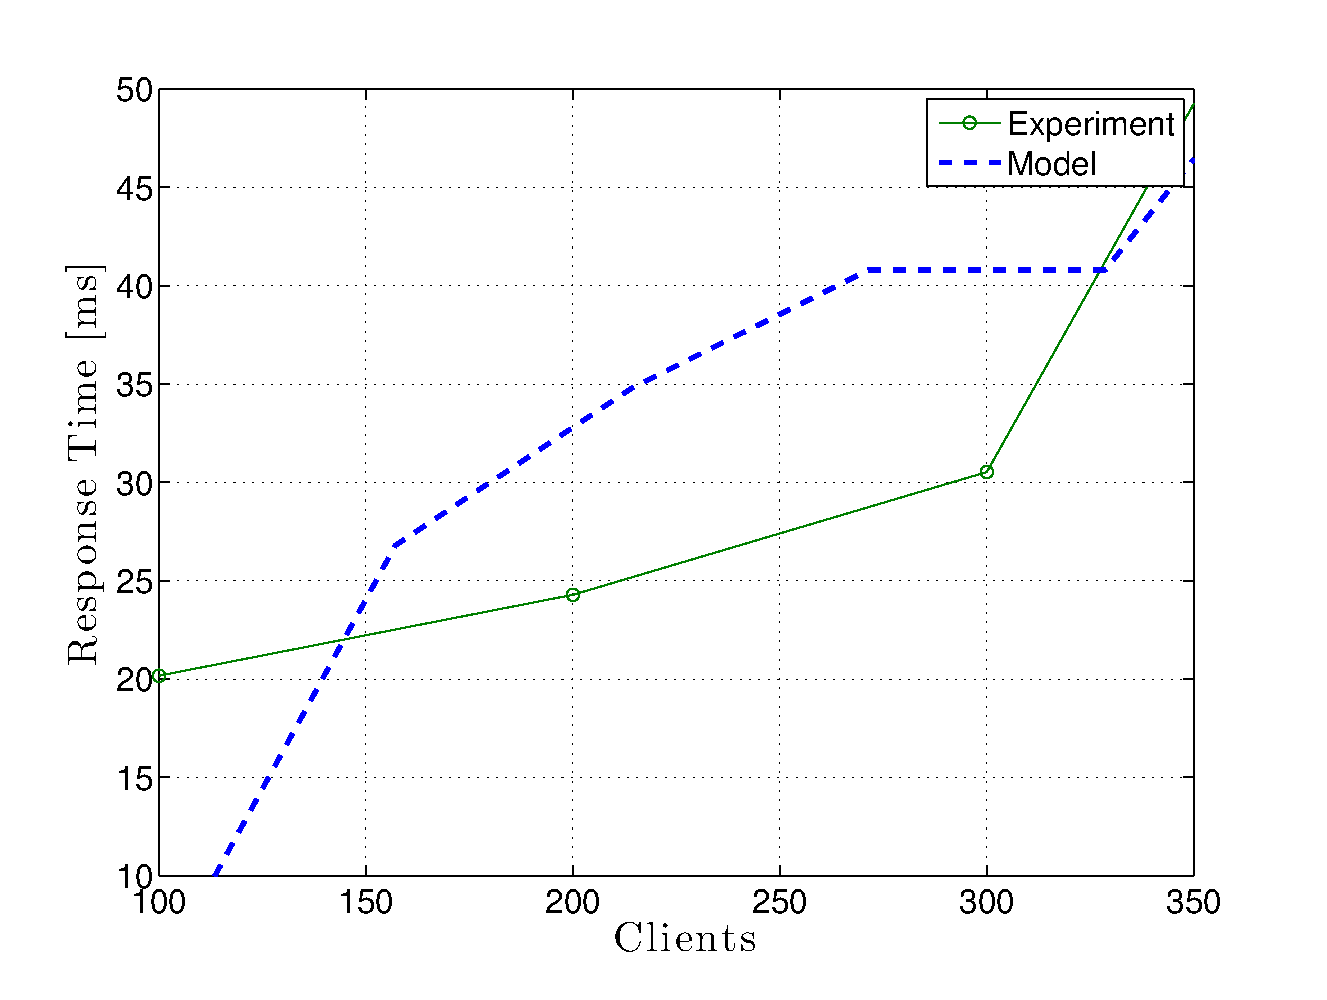
\includegraphics[width=0.8\linewidth,keepaspectratio]{secondRealAndModelError}
		\caption{Misprediction of the second model before the system reaches saturation.}
		\label{fig:secondmodelResults-error}
	\end{figure}
	\FloatBarrier

\section{Scaling}
	So one question one can ask is how does the model differentiate between scaling out and scaling up (essentially more threads vs more middleware). The answer is that since the bottle-neck is neither the working threads nor the middleware it makes no difference if the system is using 10 threads in each 8 middlewares or if it is using 80 threads in one middleware since the limiting factor is the database, given that increasing the number of threads to 80 does make the middleware the bottleneck (which is not the case in this system, but may hold in another system). This is  supported by experiments, see Figure \ref{fig:1mw80th-vs-8mw10th}. So to model a setup which corresponds to using 3 middleware with 10 threads each, set the number of CRW and Persistence servers each to 30.

	\FloatBarrier
	\begin{figure}[ch!]
		\centering
			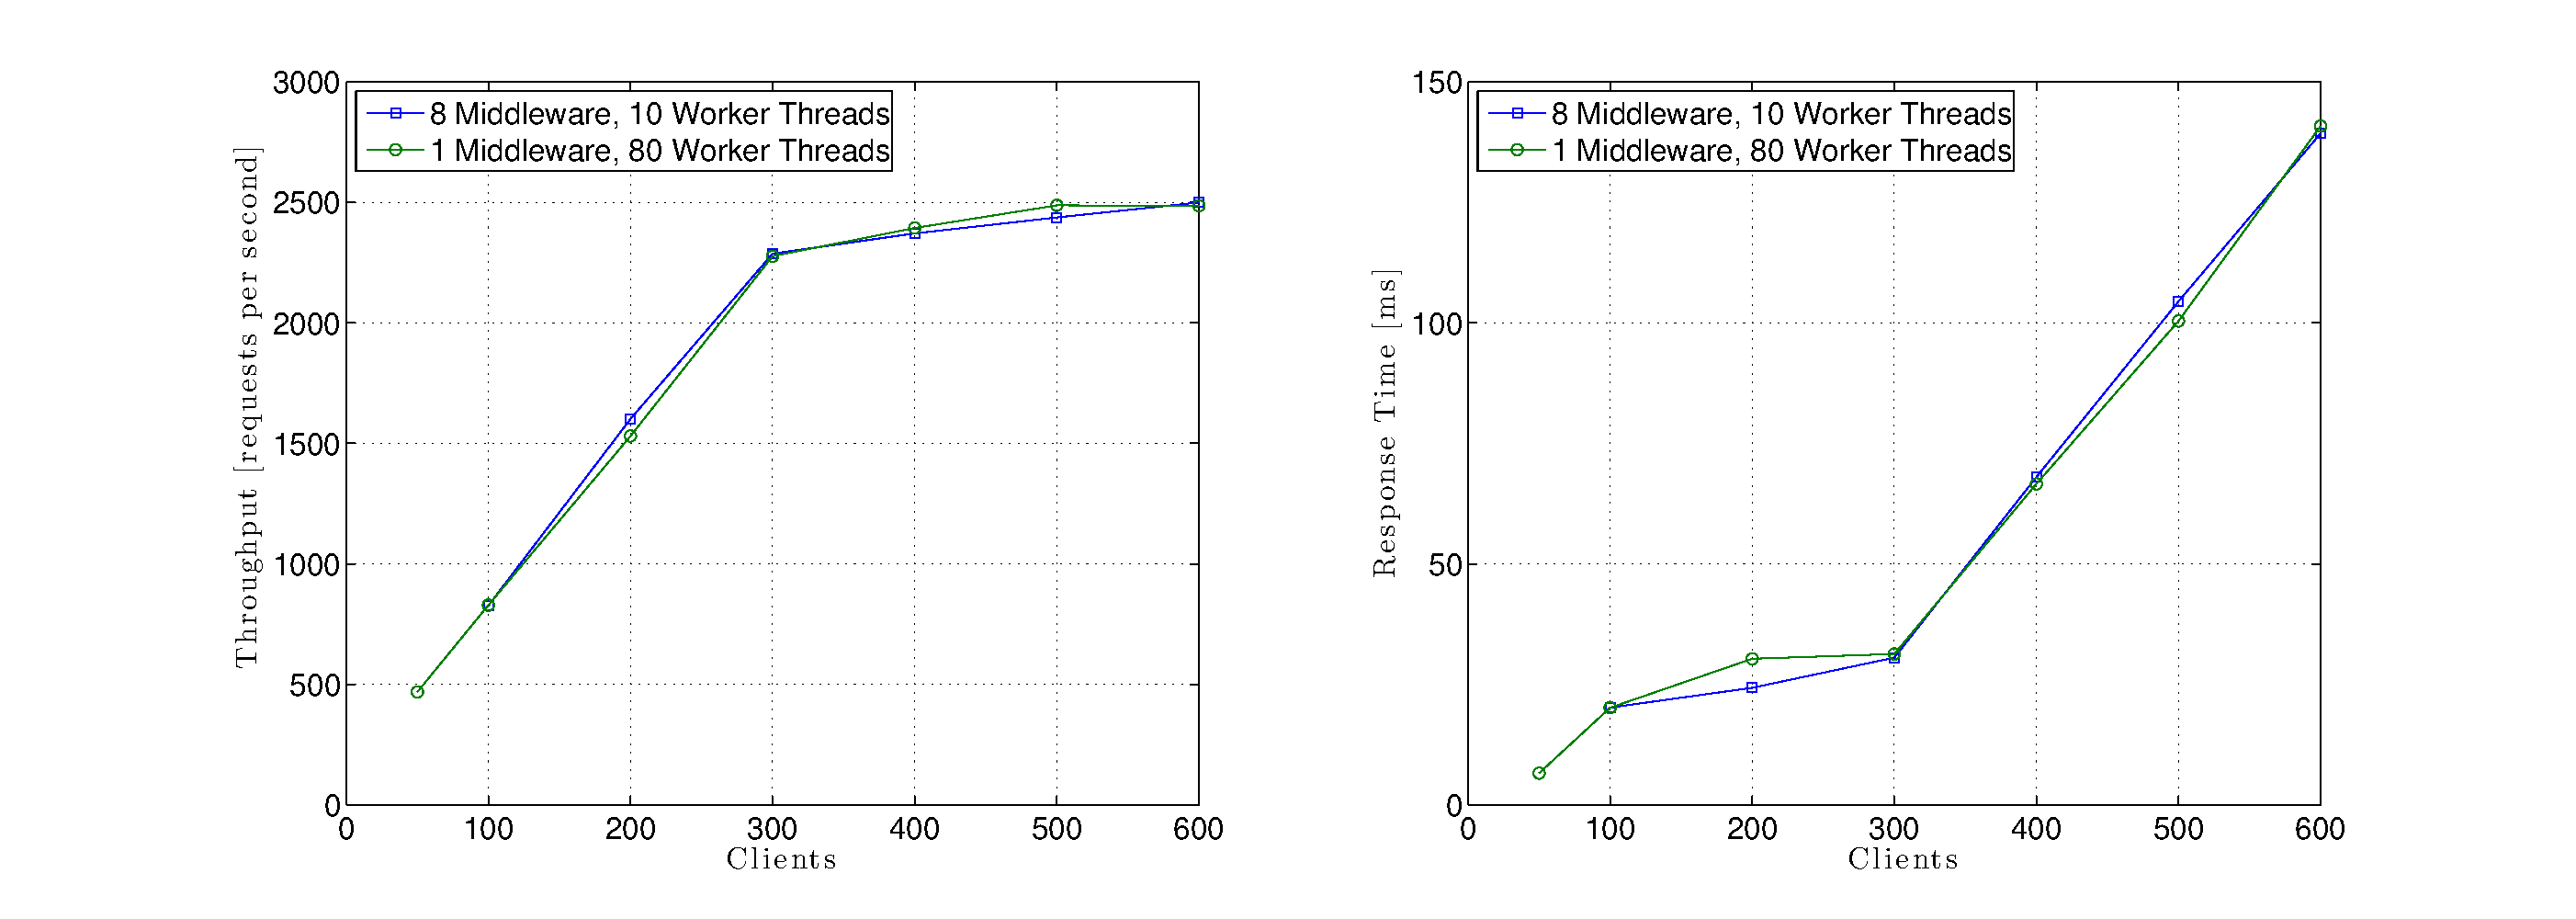
\includegraphics[width=1\linewidth,keepaspectratio]{1mw80th-vs-8mw10th}
		\caption{The througput and response time of the system while using 1 middleware and 80 worker threads (and 80 db-connections) versus using 8 middleware and 10 workers threads (and 10 db-connections) per middleware.}
		\label{fig:1mw80th-vs-8mw10th}
	\end{figure}
	\FloatBarrier


\section{Conclusion}
The final model will predict the actual performance of the real system along these parameters:
\begin{itemize}
	\item No. of Clients
	\item No. of Worker Threads
	\item Size of database connection-pool
	\item No. of Middleware
	\item Duration of Think-Time
\end{itemize}

\end{document} 
